% ELEN E6885 final project. ICML 2026 format, at most 5 pages excluding references and the
% contribution statement (context/Final Project - 2026.pdf).
% State on Nov 21, 2026 (final runs still training):
%   COMPLETE   Sections 3 (problem), 4 (approach), 5 (protocol), 6.1 and 6.2 (rules, bound, estimates)
%   DRAFT      Abstract, Sections 1 and 2: for the owner to revise
%   SKELETON   Sections 6.3 to 6.5 and 7: every \pending{} waits for the final runs or the evaluation pool
% No number from tuning seeds or development episodes is given as a result. Numbers marked
% \prov are in-sample (tuning episodes) and are replaced when the evaluation pool is opened.
% Tables and figures are written by experiments/analysis/ (make figures); do not edit them here.
\documentclass{article}

\usepackage{microtype}
\usepackage{graphicx}
\usepackage{subcaption}
\usepackage{booktabs}
\usepackage{xcolor}
\usepackage{hyperref}
\newcommand{\theHalgorithm}{\arabic{algorithm}}

% Course report, not a blind submission: the [accepted] option shows the author block.
\usepackage[accepted]{icml2026}

\usepackage{amsmath}
\usepackage{amssymb}
\usepackage{mathtools}
\usepackage[capitalize,noabbrev]{cleveref}

\newcommand{\pending}[1]{\textcolor{red}{[PENDING: #1]}}   % waits for final runs or the evaluation pool
\newcommand{\draft}[1]{\textcolor{blue}{[DRAFT: #1]}}      % for the owner to revise
\newcommand{\prov}{$^{\dagger}$}                            % provisional: in-sample, tuning episodes
\newcommand{\E}{\mathbb{E}}
% Written by experiments/analysis/fig_curves.py. Do not edit.
\newcommand{\curveseeds}{index 15, unrestricted 15, pooled 6}


\icmltitlerunning{Hiring as a Race Against Poaching}

\begin{document}

\twocolumn[
  \icmltitle{Hiring as a Race Against Poaching:\\
    Do Simple Rules Leave Anything for Reinforcement Learning?}

  \begin{icmlauthorlist}
    \icmlauthor{Author name}{cu}
  \end{icmlauthorlist}
  \icmlaffiliation{cu}{ELEN E6885 Reinforcement Learning, Columbia University, New York, USA}
  \icmlcorrespondingauthor{Author name}{author@columbia.edu}
  \icmlkeywords{reinforcement learning, sequential hiring, costly inspection, index policies, upper bounds}
  \vskip 0.3in
]

\printAffiliationsAndNotice{}

% ---------------------------------------------------------------------------------------------
\begin{abstract}
  \draft{abstract}
  An employer who interviews a candidate learns more about them but gives competitors another day
  to hire them. We study this race in a simulator of our own: three roles, sixty days, candidates
  with hidden quality, costly interviews, and competitors who take the strongest candidates
  first. Before training any agent we build three yardsticks: tuned decision rules, the exact
  optimum of a small instance, and an upper bound on the full problem. We then test two ideas with
  masked proximal policy optimization: an actor that scores each candidate separately, and a
  quality estimate corrected for the fact that candidates who are still available are a weaker
  group. Hypotheses, margins, seeds and the decision rule were fixed in a tagged pre-registration
  before the final runs. \pending{one sentence per research question, selected by the decision
  rule: rules against the bound; PPO against the exact optimum and against the best rule; index
  against unrestricted actor; naive against corrected estimate.}
\end{abstract}

% ---------------------------------------------------------------------------------------------
\section{Introduction}
\label{sec:intro}
\draft{whole section, for the owner to revise}

Hiring is a search under time pressure. Each interview makes the employer's estimate of a
candidate more accurate, but its result arrives a day later, and during that day the candidate
may accept another job. Strong candidates are the first to go. The employer therefore faces two
linked questions every day: whom to learn more about, and when to stop learning and make an
offer.

We model this as a partially observable decision problem and ask four questions.
\textbf{RQ1}: how close do simple, tuned decision rules get to the best achievable payoff?
\textbf{RQ2}: does a policy trained by reinforcement learning reach the optimum where the optimum
can be computed, and does it match or beat the best rule on the full problem?
\textbf{RQ3}: is a policy that scores each candidate separately (an index-structured policy)
enough once candidates can leave, or does an unrestricted policy do better?
\textbf{RQ4}: does correcting the quality estimate for survival change decisions and payoff?

Our contributions are these. (i) A simulator of the hiring race with fixed timing rules, in which
rules and learned agents act through the same interface (\cref{sec:problem}). (ii) Three
yardsticks built and checked before any agent was trained: tuned rules, the exact optimum of a
small instance by dynamic programming, and a Lagrangian upper bound on the full problem
(\cref{sec:yardsticks}). (iii) A controlled comparison of three actor architectures and two
quality estimates under a pre-registered protocol, with equal tuning budgets for rules and
agents and a 2\% equivalence margin fixed in advance (\cref{sec:protocol}).

We expected, and wrote down before the final runs, that the trained agents would most likely tie
the best rule on the full problem. A tie is a planned outcome here, judged by the equivalence
margin, and the yardsticks tell how much payoff any policy could still gain.
\pending{headline verdicts, one per question.}

% ---------------------------------------------------------------------------------------------
\section{Background and Related Work}
\label{sec:related}
\draft{whole section, for the owner to revise. Only sources that were opened are cited; the
reading depth of each is noted in references.bib.}

\textbf{Costly inspection.} Paying to learn the value of an option before choosing is the
subject of Pandora's problem. Recent work adds deadlines after which a box can no longer be
opened or selected and gives an approximation guarantee for that variant~\citep{qin2026}, and
allows a box to be opened in stages, a cheap partial inspection before a full
one~\citep{aouad2025}. Our candidates combine both features, staged inspection (resume, then
interviews) and limited availability, but their availability ends at a random time that depends
on their hidden quality, and several roles are filled from a stream of arrivals.

\textbf{Index policies and bounds.} For problems in which a decision maker repeatedly selects
among many items, \citet{brown2020} relax the constraint that links the items with a Lagrange
multiplier. The relaxed problem splits into one problem per item, which yields both an upper
bound on the optimal value and index-style heuristic policies. Our upper bound and our strongest
rule, the price-directed rule, follow this construction. Index structure has also been learned:
NeurWIN trains a network to output the Whittle index of a restless bandit
arm~\citep{nakhleh2021}. Our index-structured actor shares one scoring network across
candidates; unlike a Whittle index, its scores are trained end to end by policy gradient and are
not required to be an index in the technical sense.

\textbf{Learning method.} We use proximal policy optimization~\citep{schulman2017} with invalid
actions masked out of the policy~\citep{huang2022}, in the Stable-Baselines3
implementation~\citep{raffin2021}. The pooled actor adds a permutation-invariant summary of the
candidate set in the manner of Deep Sets~\citep{zaheer2017}. Our reporting follows the advice of
\citet{agarwal2021} to treat the training seed as the unit of analysis and to report interval
estimates.

\textbf{Selection by departure.} That the candidates who remain available are a selected,
weaker group is a known effect in duration models. \pending{cite a source for dynamic selection
(frailty) once it has been opened; none has been yet.}

\textbf{Novelty.} To our knowledge, and within a literature search completed on 12 November
2026 \draft{state the search scope: databases and query terms; the search record is
notes/prior\_art\_and\_novelty.md}, no published work trains and evaluates a learned policy for
this combined setting: sequential costly interviews, quality-dependent departures, declining
acceptance and a deadline, measured against an exact optimum and an upper bound. We do not claim
to be the first to learn index policies, to show that index policies can fail, or to observe
that survival biases a quality estimate.

% ---------------------------------------------------------------------------------------------
\section{Problem and Simulator}
\label{sec:problem}

\textbf{The task.} A firm must fill $m$ roles within $T$ days. Each day a Poisson number of
candidates arrives, with mean $\lambda$. Candidate $i$ has a hidden quality
$q_i \sim \mathcal{N}(0,1)$ that is never observed. On arrival the firm sees a noisy resume
score $q_i + \sigma_R \varepsilon$. An interview costs $c$ and returns another noisy score
$q_i + \sigma_I \varepsilon'$. The firm may make an offer to any candidate in its pool. An offer
made after the candidate has waited $d$ days is accepted with probability
$a_0 e^{-\beta d}$; a candidate who declines leaves. Each night every waiting candidate is hired
elsewhere (``poached'') with probability
\begin{equation}
  h(q_i) = \min\bigl(1,\; h_0 e^{\kappa q_i}\bigr), \qquad \kappa > 0,
  \label{eq:hazard}
\end{equation}
so stronger candidates leave sooner. The payoff of an episode is the total quality of the
accepted hires minus the interview costs, and the firm maximises its expectation. The episode ends
when all roles are filled or after day $T$.

\textbf{Why it is a race.} Waiting has two prices. An interview improves the estimate of $q_i$,
but its result arrives the next morning, after one more night of poaching and with a lower
acceptance probability. And by \cref{eq:hazard} the candidates who are still available are, on
average, weaker than their scores suggest (\cref{sec:belief}).

\textbf{Order of a day.} The results depend on the timing rules, so we fix them: (1) yesterday's
interview results are revealed; (2) new candidates arrive; (3) the firm makes offers, one at a
time, each resolved before the next; (4) the firm chooses interviews, after which no further
offer is possible that day; (5) poaching happens overnight. A candidate can be interviewed at
most once per day and at most three times in total, at most $K$ interviews take place per day,
and none on the last day, when a result could no longer be used. A candidate interviewed today
can therefore receive an offer tomorrow at the earliest, and an interview result is lost if the
candidate is poached that night. Reaching the deadline ends the episode as a terminal state, not
as a time-limit truncation, because the deadline is part of the task.

\textbf{Decision interface.} The policy acts one step at a time: it picks one of the $N = 10$
shown candidates and either interviews or makes an offer, or it ends the day. That is one choice
among $2N + 1$ actions, with invalid choices masked. The shown candidates are the $N$ with the
highest resume-and-interview estimate, in that order, for every policy we compare; rules and
learned agents act through this same view. The observation holds, for each shown candidate, the
quality estimate, the number of interview results seen, the days waited and whether the candidate
was interviewed today, and, for the firm, the days left, the roles left, the interview slots left
today, the pool size and whether offers are still open today. Features are scaled by fixed
constants inside the simulator, identically for every candidate slot.

\begin{table}[t]
  \caption{The two parameter sets. Stress is run at five pressure levels: no pressure
    ($h_0 = 0$, $\beta = 0$) and $h_0 \in \{0, 0.02, 0.05, 0.10\}$ with $\beta = 0.03$; the
    primary setting is $h_0 = 0.05$.}
  \label{tab:scenarios}
  \centering
  \begin{small}
    \begin{tabular}{lcc}
      \toprule
      Parameter & Stress & Calibrated \\
      \midrule
      Horizon $T$, roles $m$ & 60, 3 & 60, 3 \\
      Arrivals per day $\lambda$ & 1.5 & 1.5 \\
      Interviews per day $K$ & 3 & 3 \\
      Resume noise $\sigma_R$ & 1.5 & 2.4 \\
      Interview noise $\sigma_I$ & 1.0 & 2.2 \\
      Interview cost $c$ & 0.05 & 0.05 \\
      Base acceptance $a_0$ & 0.90 & 0.80 \\
      Acceptance decay $\beta$ & 0.03 & 0.003 \\
      Poaching level $h_0$ & 0 to 0.10 & 0.02 \\
      Quality slope $\kappa$ & 0.6 & 0.6 \\
      \bottomrule
    \end{tabular}
  \end{small}
\end{table}

\textbf{Two parameter sets} (\cref{tab:scenarios}). The \emph{stress} scenario is our main test
bed; its acceptance decay and its upper poaching levels are harsher than hiring benchmarks
support, and we label it as such. The \emph{calibrated} scenario moves five values toward
published recruiting statistics. The horizon matches a median time to fill of 60 to 61 days at
large employers~\citep{shrm2025}. Base acceptance and its decay are set so that realised offer
acceptance falls inside the 76 to 84\% reported by \citet{ashby2024} and \citet{gem2025}. The
poaching level is our inference from the shares of candidates who say they would disengage after
one week (12\%) and one month (36\%)~\citep{cronofy2024}. The two noise levels are our mapping,
$r = 1/\sqrt{1 + \sigma^2}$, of the validities reported by \citet{sackett2023} for structured
interviews ($r = .42$) and empirically keyed biodata ($r = .38$, our stand-in for a resume). The
quality slope $\kappa$, the exponential forms and the interview cost have no empirical basis.

\textbf{A small instance that can be solved exactly.} With one role, twelve days, at most one
arrival per day (probability 0.6), one interview per day, at most two interviews per candidate,
at most two candidates in the pool and scores reported in three bins, the belief state is finite
and the optimal policy follows from dynamic programming (\cref{sec:yardsticks}). When a third
candidate arrives, the one with the lowest estimate is dropped automatically. The same simulator
class runs this instance, so it is a known-answer test for every learned agent.

% ---------------------------------------------------------------------------------------------
\section{Approach}
\label{sec:methods}

\subsection{Survival-aware estimate}
\label{sec:belief}
After the resume score $x$ and $n$ interview scores $y_1, \dots, y_n$, the usual (``naive'')
posterior of a candidate's quality is Gaussian with
\begin{equation}
  s_n^2 = \Bigl(1 + \tfrac{1}{\sigma_R^2} + \tfrac{n}{\sigma_I^2}\Bigr)^{-1}, \quad
  \mu_n = s_n^2 \Bigl(\tfrac{x}{\sigma_R^2} + \tfrac{1}{\sigma_I^2}\textstyle\sum_j y_j\Bigr).
  \label{eq:naive}
\end{equation}
It ignores that the candidate is still available. A candidate who is still available after $d$
nights of poaching has the posterior
\begin{equation}
  p(q \mid x, y_{1:n}, d) \;\propto\;
  \mathcal{N}(q;\, \mu_n, s_n^2)\,\bigl(1 - h(q)\bigr)^{d},
  \label{eq:survival}
\end{equation}
whose mean $\hat q(\mu_n, n, d)$ is the \emph{survival-aware} estimate. The triple
$(\mu_n, n, d)$ is a sufficient statistic, and the mean is a one-dimensional integral that we
compute by Gauss--Hermite quadrature. The correction is not small: under the stress noise
levels, a candidate with a resume-only naive estimate of 1.0 who is still available after seven
days has a survival-aware estimate of 0.88, 0.72 and 0.48 at $h_0 = 0.02$, $0.05$ and $0.10$.
The observation always contains the days waited, so an agent given the naive estimate could in
principle learn the correction itself; hypothesis H4b tests whether supplying it matters.

\subsection{Agents}
\label{sec:agents}
All agents are trained with proximal policy optimization with action masking, one process per
run, and share the same critic: a fully connected network on the whole observation. They differ
only in the actor. Write $x_i$ for the features of shown candidate $i$ and $g$ for the firm's
features.

\textbf{Unrestricted actor.} A fully connected network maps the whole observation to the
$2N + 1$ action scores. It can represent any interaction between candidates.

\textbf{Index-structured actor.} One network $f_\theta$, shared by all candidates, maps
$(x_i, g)$ to two scores, one for interviewing and one for making an offer to candidate $i$. A
second small network maps $g$ alone to the score for ending the day. The score of one candidate
therefore cannot depend on any other candidate. Because $g$ contains the clock and the roles
left, this is a time- and state-dependent priority rule, richer than a static index.

\textbf{Pooled actor.} As the index-structured actor, but every candidate's input, and the
end-day input, also carries a summary of the pool: the mean over the present candidates of a
learned embedding of $(x_i, g)$, and the number present. Weights are still shared. This actor
differs from the index-structured one only in pool awareness and from the unrestricted one only
in symmetry, which separates the two possible reasons for a gap between them.

Agents are scored by their most probable valid action (greedy), both for the learning curves and
for final scoring. The reward is the unshaped payoff.

\subsection{Yardsticks}
\label{sec:yardsticks}
\textbf{Rules.} Four families of threshold rules of growing flexibility act on a quality
estimate $e$: a \emph{static bar} (offer if $e$ exceeds a constant); a \emph{falling bar} that
decreases with time and with the number of open roles; a \emph{one-interview} rule that
interviews candidates above a lower bar and offers after the result; and a rule with \emph{up to
two interviews}. Each family contains the ones before it. On the last day every rule offers to
any candidate with a positive estimate. The fifth rule, the \emph{price-directed} rule, comes
from the bound below: at every decision it finds the price of a hire that the relaxation would
charge in the current state and lets each candidate take its own best action at that price,
offers first. It has two tuned parameters, a multiplier on that price and a price per interview.
Every rule exists in two versions, using the naive or the survival-aware estimate.

\textbf{Exact optimum on the small instance.} A candidate's state is its resume bin, its
interview outcome counts and its days waited; the pool is a sorted tuple of such states. Backward
induction over (day, pool), through the offer phase, the interview phase and the night, gives the
optimal expected payoff, $0.6333$. The same backward pass with a trained agent's greedy action in
place of the maximum gives that agent's expected payoff exactly, with no sampling, which is how
agents are scored on this instance.

\textbf{Upper bound on the full problem.} Two constraints tie candidates together: at most $m$
hires, and at most $K$ interviews per day. Following \citet{brown2020}, we charge a price
$z \ge 0$ per hire and $\ell \ge 0$ per interview and drop both constraints. Every policy of the
real problem earns at least as much in the priced problem, which splits into independent
one-candidate problems, so the optimal payoff $V^\star$ satisfies
\begin{equation}
  V^\star \le \min_{z,\ell \ge 0} \Bigl[ m z + \ell K (T{-}1) + \lambda \textstyle\sum_{t=1}^{T} F_t(z, \ell) \Bigr],
  \label{eq:bound}
\end{equation}
where $F_t(z, \ell)$ is the optimal value of one candidate arriving on day $t$ who yields
$q - z$ if hired and pays $c + \ell$ per interview. Each $F_t$ is a small dynamic program on
$(\mu_n, n, d)$ under the survival-aware posterior. The relaxation also drops the
offer-then-interview order and the $N$-candidate view; each of these can only raise the bound.
A finer numerical grid lowers the bound by less than $0.006$ at every setting.

The bound may be far from tight. On the small instance, where the optimum is known exactly, the
bound is 0.862 against an optimum of 0.633, that is 36\% above it. The distance between the best
policy and the bound on the full problem may therefore be mostly slack in the bound rather than
payoff left unearned, and we do not read that distance as a shortfall of any policy.

% ---------------------------------------------------------------------------------------------
\section{Experimental Protocol}
\label{sec:protocol}
The protocol was written down in a pre-registration file, tagged in the repository on
21~November 2026 before any final training seed was run. This section restates it.

\textbf{Hypotheses.} H1a: on the small instance the best tuned rule reaches at least 95\% of the
exact optimum. H1b: on the full problem the best tuned rule reaches 85 to 91\% of the upper
bound, and the shortfall grows with $h_0$. H2a: PPO is within 2\% of the exact optimum on the
small instance. H2b: on the full problem PPO's payoff is at least that of the best tuned rule.
H3: the unrestricted minus the index-structured agent is within the 2\% margin at $h_0 = 0$ and
grows with $h_0$. H4a: inside a fixed rule, replacing the naive by the survival-aware estimate
changes decisions on a measurable share of candidate-days and raises payoff at $h_0 \ge 0.05$.
H4b: for PPO, which observes the days waited, the two estimates give payoffs within 2\%, and the
survival-aware agent reaches a given payoff in fewer steps.

\textbf{Seeds and episodes.} Four pools are kept apart. Tuning uses training seeds 101 to 103 and
4{,}000 tuning episodes. Final runs use training seeds 1001 to 1015, fifteen per condition, and
are scored on 10{,}000 evaluation episodes that nothing was tuned on. A third set of episodes
serves tests and learning curves only and is never reported as a result. No seed is dropped.
Each episode seed fixes arrivals, qualities, noise, departures and acceptance draws per
candidate, so every policy meets the same candidates: all comparisons are paired by episode.

\textbf{Metric and decision rule.} The metric is the mean unshaped payoff over the evaluation
episodes. The unit of analysis is the training seed. For a comparison we take the 95\% bootstrap
interval of the mean paired difference and a margin of 2\% of the comparator's payoff. If the
interval lies inside the margin the verdict is \emph{equivalent}; otherwise, if it lies above
zero, \emph{better}; below zero, \emph{worse}; anything else is \emph{inconclusive} and is
reported as such. Equivalence takes precedence. We report interquartile means over
seeds~\citep{agarwal2021}, Welch's test alongside, and a multiplicity correction over the
primary comparisons. The primary comparison is PPO against the best tuned rule at $h_0 = 0.05$.

\textbf{Equal tuning budgets.} Each rule family gets 40 parameter vectors per estimate and
setting, each scored on all tuning episodes; a threshold family is in addition scored at the
best vector of each family it contains. Each actor gets 40 hyperparameter configurations from a
seeded random search (the same 40 for every actor), trained with the three tuning seeds for 30\%
of the final length; the five best are retrained at full length and the best of those is frozen.
PPO thus never gets less than its comparator. A 360-vector search at the primary setting checks
that the rules are not under-tuned: if the best rule gained more than the margin, the stronger
rule would become the comparator.

\textbf{Training length and convergence.} The index-structured actor trains for 3 million steps
and the other two for 10 million, fixed by rules set in advance: doubling the length had to
change the payoff by less than 1\%. Every run logs payoff, policy loss, value loss, entropy,
approximate KL divergence and clip fraction. A curve is called flat only if the 95\% interval of
its change over the last fifth of training lies inside $\pm 1\%$ of the final payoff.

\textbf{Final runs and ablations.} Each actor is trained at seven settings (the small instance,
no pressure, four poaching levels, calibrated) with the survival-aware estimate, and at the
primary setting also with the naive estimate (H4b): 360 runs. Ablations change one thing at a
time from the frozen index-structured configuration at the primary setting, three seeds each:
discount, entropy coefficient, learning rate and rollout length (two other values each),
potential-based reward shaping, and an end-day score that also reads the pool summary.

\textbf{Known-answer tests.} Before the final runs each actor had to reach 98\% of the exact
optimum on the small instance, copy the exact optimal policy by supervised learning, and the
bound had to exceed every evaluated policy at every setting.

\textbf{Recorded departures.} (i) Hyperparameters were tuned at the primary setting only, not
also on the small instance; the small-instance test was rerun on the frozen configurations
instead. (ii) After tuning, a flaw in the rule search was found and fixed before the tag: a wider
rule family could score below a family it contains, which had overstated two gaps between the
estimates. (iii) The training code gained the ablation options after the tag, while final runs
were in progress, so runs record different code versions; the default training path gives
bit-identical weights before and after the change. \pending{any further deviation, including
the seed cutoff rule if it fires.}

% ---------------------------------------------------------------------------------------------
\section{Results}
\label{sec:results}

\subsection{Rules against the bound (RQ1)}
\label{sec:rq1}
\begin{table}[t]
  \caption{Upper bound and best tuned rule of each family (better of the two estimates). Last
    column: best rule as a percentage of the bound. The bound involves no sampling and is final.
    \prov Rule scores are on the 4{,}000 tuning episodes the rules were fitted on, so they are
    biased upward; evaluation-pool values will replace them.}
  \label{tab:rules}
  \centering
  \begin{footnotesize}
    % Written by experiments/analysis/table_rules.py. Do not edit.
\begin{tabular}{@{}l@{\hskip 4pt}c@{\hskip 4pt}c@{\hskip 4pt}c@{\hskip 4pt}c@{\hskip 4pt}c@{\hskip 4pt}c@{\hskip 4pt}c@{}}
\toprule
Setting & Bound & Static & Falling & 1 int. & 2 int. & Price & \% \\
\midrule
No press. & 4.34 & 3.54 & 3.54 & 4.04 & \textbf{4.05} & 4.04 & 93 \\
$h_0{=}0$ & 4.29 & 3.39 & 3.40 & 3.86 & 3.87 & \textbf{3.91} & 91 \\
$h_0{=}0.02$ & 4.16 & 3.25 & 3.33 & 3.73 & 3.73 & \textbf{3.77} & 91 \\
$h_0{=}0.05$ & 3.98 & 3.21 & 3.30 & 3.53 & 3.56 & \textbf{3.59} & 90 \\
$h_0{=}0.10$ & 3.77 & 3.17 & 3.28 & 3.28 & 3.28 & \textbf{3.41} & 91 \\
Calibrated & 2.65 & 2.17 & 2.22 & 2.35 & 2.35 & \textbf{2.38} & 90 \\
\bottomrule
\end{tabular}

  \end{footnotesize}
\end{table}

\Cref{tab:rules} gives the bound and the tuned rules. Three observations hold on the tuning
episodes\prov. First, interviews are worth their cost when there is time: without pressure the
interviewing rules gain about 0.5 over the rules that offer on the resume alone, and at
$h_0 = 0.10$ the tuned one- and two-interview rules stop interviewing and coincide with the
falling bar. Second, the price-directed rule is the best rule at every setting with pressure and
within 0.01 of the best without. Third, the best rule is at 90 to 93\% of the bound. That is at
or above the upper end of the 85 to 91\% predicted in H1b, and the share does not fall steadily
with $h_0$, against the second half of H1b. \pending{H1b verdict on the evaluation episodes, with
intervals.} Because the bound is loose (\cref{sec:yardsticks}), the remaining 7 to 10\% is an
upper limit on what any policy, learned or not, could add to the best rule.
\pending{H1a: best tuned rule on the small instance against the exact optimum $0.6333$. The
rules have not yet been tuned on the small instance.}

\subsection{The two estimates inside a rule (H4a)}
\label{sec:h4a}
\begin{table}[t]
  \caption{Payoff with the survival-aware estimate minus payoff with the naive estimate, for the
    same rule family, each version tuned separately. At $h_0 = 0$ the two estimates are equal,
    so that column shows the noise of the parameter search. \prov Tuning episodes; unpaired.}
  \label{tab:belief}
  \centering
  \begin{footnotesize}
    % Written by experiments/analysis/table_belief.py. Do not edit.
\begin{tabular}{@{}l@{\hskip 5pt}c@{\hskip 5pt}c@{\hskip 5pt}c@{\hskip 5pt}c@{\hskip 5pt}c@{}}
\toprule
 & \multicolumn{4}{c}{Stress, $h_0$} & \\
\cmidrule(lr){2-5}
Rule family & $0$ & $0.02$ & $0.05$ & $0.10$ & Calib. \\
\midrule
Static bar & $-0.003$ & $+0.023$ & $+0.031$ & $+0.035$ & $+0.047$ \\
Falling bar & $+0.002$ & $+0.080$ & $+0.104$ & $+0.100$ & $+0.096$ \\
One interview & $+0.014$ & $+0.064$ & $+0.098$ & $+0.100$ & $+0.226$ \\
Two interviews & $-0.014$ & $+0.042$ & $+0.043$ & $+0.100$ & $+0.193$ \\
Price-directed & $-0.014$ & $+0.019$ & $+0.030$ & $+0.048$ & $+0.072$ \\
\bottomrule
\end{tabular}

  \end{footnotesize}
\end{table}

\Cref{tab:belief} compares the two estimates inside each rule family\prov. Without poaching the
estimates coincide and the differences, at most 0.014 in size, measure only the noise of
separate tuning. With poaching the survival-aware version scores higher in every family at
every level, by more than that noise: by 0.03 to 0.10 at the primary setting and by up to 0.23
in the calibrated scenario, where signals are noisier and the estimate matters more. The
direction agrees with H4a. \pending{H4a verdict: paired differences with 95\% intervals on the
evaluation episodes, and the share of candidate-days on which the two versions of a rule choose
differently.} A correction found before the tag belongs here: an earlier search had reported
calibrated gaps of $+0.24$ and $+0.32$ for the falling-bar and one-interview rules; these were
overstated because the naive search had missed a simpler rule it contains
(\cref{sec:protocol}).

\subsection{Learned agents (RQ2, RQ3, H4b)}
\label{sec:ppo}
\begin{figure*}[t]
  \centering
  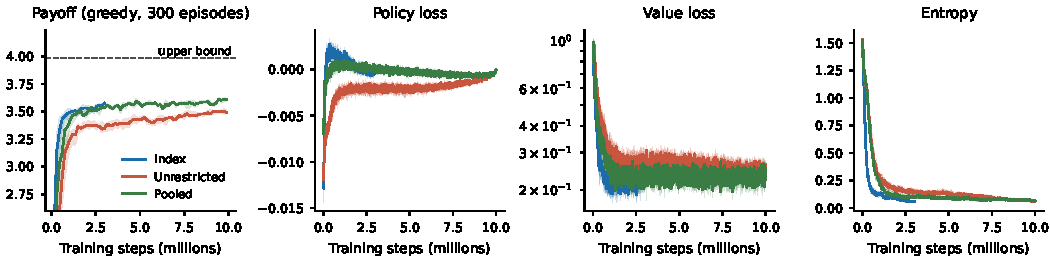
\includegraphics[width=\textwidth]{figures/curves.pdf}
  \caption{Learning curves of the final runs at the primary setting ($h_0 = 0.05$): median and
    interquartile band over training seeds (\curveseeds\ finished so far; \pending{15 each}).
    The payoff panel uses 300 fixed curve episodes, which are not evaluation episodes: the
    figure documents convergence and is not a result. \pending{reference lines for the random
    policy and the best rule on the same episodes.}}
  \label{fig:curves}
\end{figure*}

\Cref{fig:curves} shows the learning curves. \pending{plateau test per actor: flat,
inconclusive or changing, under the $\pm 1\%$ rule.}

\begin{table}[t]
  \caption{\pending{Main table: mean payoff on the 10{,}000 evaluation episodes, interquartile
    mean over 15 training seeds with 95\% intervals, as a percentage of the bound (and of the
    exact optimum on the small instance).}}
  \label{tab:main}
  \centering
  \begin{footnotesize}
    \begin{tabular}{@{}lccccc@{}}
      \toprule
      Setting & Rule & Index & Unrestr. & Pooled & Bound \\
      \midrule
      Small instance & -- & -- & -- & -- & 0.862 \\
      No pressure & -- & -- & -- & -- & 4.34 \\
      $h_0 = 0$ & -- & -- & -- & -- & 4.29 \\
      $h_0 = 0.02$ & -- & -- & -- & -- & 4.16 \\
      $h_0 = 0.05$ & -- & -- & -- & -- & 3.98 \\
      $h_0 = 0.10$ & -- & -- & -- & -- & 3.77 \\
      Calibrated & -- & -- & -- & -- & 2.65 \\
      \bottomrule
    \end{tabular}
  \end{footnotesize}
\end{table}

For each hypothesis the sentence below is the one the decision rule selects; the other three are
kept in the source as comments until the numbers are in.

\textbf{H2a, small instance.} \pending{Select one per actor.
\emph{Equivalent:} the agent's exact payoff is within 2\% of the optimum ($x$\% of $0.6333$).
\emph{Worse:} the agent falls short of the optimum by more than the margin.
\emph{Inconclusive:} seeds fall on both sides of the 98\% mark.
(\emph{Better} cannot occur: the optimum is exact.)}
% Equivalent: Every actor reaches the exact optimum within the 2% margin: ...
% Worse:      The <actor> actor stays more than 2% below the exact optimum: ...
% Inconclusive: ...

\textbf{H2b, PPO against the best rule, primary setting.} \pending{Select one.
\emph{Equivalent:} the interval of the paired difference lies inside $\pm 2\%$ of the rule's
payoff: PPO ties the best rule, the planned outcome.
\emph{Better:} the interval lies above zero and outside the margin: PPO beats the best rule by
$x$.
\emph{Worse:} the interval lies below zero and outside the margin: PPO falls short of the best
rule by $x$; \cref{sec:hurdles} examines why.
\emph{Inconclusive:} the interval crosses the margin; we report the interval and draw no
verdict.}

\textbf{H3, unrestricted minus index-structured actor.} \pending{Select one per poaching level,
and state whether the difference grows with $h_0$.
\emph{Equivalent:} index structure costs nothing measurable at this level.
\emph{Better:} the unrestricted actor gains $x$ over the index-structured one.
\emph{Worse:} the unrestricted actor scores below the index-structured one by $x$, which points
to optimisation difficulty, not to a limit of index structure.
\emph{Inconclusive:} no verdict. The pooled actor then tells whether a gap comes from pool
awareness or from symmetry.}

\textbf{H4b, naive against survival-aware estimate in the observation.} \pending{Select one per
actor, and report steps to a fixed payoff.
\emph{Equivalent:} the agent recovers the correction from the days waited.
\emph{Better / worse:} supplying the corrected estimate changes the final payoff by $x$.
\emph{Inconclusive:} no verdict.}

\subsection{Tuning and ablations}
\label{sec:ablations}
\pending{Tuning table: the frozen configuration of each actor and the spread of the 40 search
configurations (tuning seeds; reported as sensitivity evidence, not as results). Ablation table:
payoff change against the frozen index-structured configuration for discount, entropy
coefficient, learning rate, rollout length, reward shaping and the end-day variant, three seeds
each, with intervals. Runs start after the main runs.}

\subsection{Hurdles and failure modes}
\label{sec:hurdles}
\pending{Written after the final evaluation. Tested mechanisms are kept apart from conjecture.
Planned content: (a) headroom: rule, agents and bound per setting; (b) where agents and the best
rule differ: mistakes counted by type (offer too early, interview wasted, candidate lost
overnight) on evaluation episodes, and priced exactly on the small instance; (c) task features
that make learning hard here: long horizon with terminal-heavy reward, payoff variance from
acceptance and poaching draws, few interview slots; (d) which of these the ablations moved.}

% ---------------------------------------------------------------------------------------------
\section{Limitations and Conclusion}
\label{sec:conclusion}
\pending{Conclusion: one paragraph, one verdict per research question.}

\textbf{Limitations.} The results are for one simulator. The quality slope, the exponential
forms and the interview cost are not calibrated. The exact optimum is known only on a small
instance, and the upper bound is loose, so the distance to the bound overstates what is left to
gain. The calibrated scenario matches published offer-acceptance rates (79\% realised under the
best rule on the tuning episodes, against a benchmark of 76 to 84\%~\citep{ashby2024,gem2025})
but not interview volume: the best rule interviews 3.6 times per hire, where the benchmark is
about 20~\citep{gem2025}. Interviews in our model are therefore far more informative per unit
cost than real ones, and the calibrated results should not be read as quantitative predictions
about hiring practice. \pending{limitations that the final results add.}

% ---------------------------------------------------------------------------------------------
\section*{Reproducibility}
Code, configurations, the pre-registration and every run's logs are at
\url{https://github.com/EliasHaddad00/Hiring_RL_Research} (tag \texttt{preregistration}). Trained
models are attached to the release \texttt{final-models} and verified by checksum after
download. \texttt{make figures} regenerates every table and figure from saved results.
\pending{tag of the submitted version.}

\bibliography{references}
\bibliographystyle{icml2026}

\section*{Contributions of Team Members}
\pending{statement by the owner.}

% ---------------------------------------------------------------------------------------------
\newpage
\appendix
\onecolumn
\section{Supplementary Material: Detailed Methodology}
\label{sec:supplement}
The assignment allows the detailed methodology of an algorithm as supplementary material. Nothing
here is needed to read the results.

\textbf{Hyperparameters.} \Cref{tab:hyper} lists the frozen configuration of each actor and the
search ranges. All runs use 8 environments in one process, a learning rate that falls linearly to
zero, value coefficient 0.5 and gradient clipping at 0.5.

\begin{table}[h]
  \caption{Frozen hyperparameters (chosen on tuning seeds 101 to 103) and search ranges.}
  \label{tab:hyper}
  \centering
  \begin{small}
    \begin{tabular}{lccc}
      \toprule
      Hyperparameter & Index-structured & Unrestricted, pooled & Search range \\
      \midrule
      Training steps & 3 million & 10 million & fixed in advance \\
      Rollout length per environment & 512 & 512 & 256, 512, 1024, 2048 \\
      Minibatch size & 64 & 256 & 64 to 1024 (powers of two) \\
      Epochs per update & 5 & 10 & 4, 5, 10 \\
      Discount & 1.0 & 1.0 & 0.99, 0.995, 0.999, 1.0 \\
      Clip range & 0.2 & 0.1 & 0.1, 0.2, 0.3 \\
      Hidden width & 256 & 256 & 64, 128, 256 \\
      Learning rate (start) & $6.6 \times 10^{-4}$ & $2.3 \times 10^{-4}$ & $10^{-4}$ to $10^{-3}$ (log) \\
      Entropy coefficient & $5.1 \times 10^{-3}$ & $7.0 \times 10^{-3}$ & $10^{-3}$ to $3 \times 10^{-2}$ (log) \\
      GAE parameter & 0.919 & 0.926 & 0.90 to 0.98 \\
      \bottomrule
    \end{tabular}
  \end{small}
\end{table}

\textbf{One-candidate problem behind the bound.} State: naive mean $\mu_n$ (on a grid of 181
points with linear interpolation), interviews seen $n$, days waited $d$, days remaining. Actions:
pass; offer, worth $a_0 e^{-\beta d}(\hat q - z)$; interview, allowed if a day remains and $n$ is
below the cap, at cost $c + \ell$, with the result seen next morning and lost if the candidate is
poached that night; wait. Expectations use the survival-aware posterior of \cref{eq:survival}. On
the small instance the tables are exact; on the full problem the minimising interview price is
$\ell = 0$ at every setting.

\textbf{Reward shaping (ablation).} Potential-based, with potential
$\Phi(s) = \sum \max(\hat q_i, 0)$ over the $k$ candidates in the pool with the highest shown
estimate, $k$ being the number of open roles, and $\Phi = 0$ in terminal states. The training
reward is $r + \gamma \Phi(s') - \Phi(s)$. All reported payoffs are unshaped.

\textbf{Seed cutoff.} If the main runs are not finished by the end of 4 December, a setting not
yet started is run with seeds 1001 to 1010 only and reported as a deviation. The cutoff is a
date and never depends on results. The primary setting and the H4b runs always get 15 seeds.

\end{document}
